% Day 1: Why Digital Finance? -- From Friction to Innovation
% Complete Beamer slides for Digital Finance course
\documentclass[11pt,aspectratio=169]{beamer}
\usetheme{Madrid}

% ======================= PACKAGES =======================
\usepackage{graphicx}
\usepackage{booktabs}
\usepackage{adjustbox}
\usepackage{multicol}
\usepackage{amsmath}
\usepackage{amssymb}
\usepackage{tikz}
\usetikzlibrary{arrows,shapes,positioning,shadows,trees}
\usepackage{listings}
\usepackage{xcolor}

% ======================= COLOR DEFINITIONS =======================
% Primary color scheme: Blue/Teal for Digital Finance
\definecolor{dfblue}{RGB}{0,102,204}
\definecolor{dfteal}{RGB}{0,153,153}
\definecolor{dfcyan}{RGB}{51,187,204}
\definecolor{dflightblue}{RGB}{153,204,255}
\definecolor{dflightblue2}{RGB}{173,214,255}
\definecolor{dflightblue3}{RGB}{193,224,255}
\definecolor{dflightblue4}{RGB}{213,234,255}

% Accent colors for finance applications
\definecolor{dfgreen}{RGB}{44, 160, 44}
\definecolor{dfred}{RGB}{214, 39, 40}
\definecolor{dforange}{RGB}{255, 127, 14}
\definecolor{dfgray}{RGB}{127, 127, 127}

% Utility colors
\definecolor{lightgray}{RGB}{240, 240, 240}
\definecolor{midgray}{RGB}{180, 180, 180}
\definecolor{codebg}{RGB}{245, 245, 245}

% ======================= THEME CUSTOMIZATION =======================
% Apply Digital Finance color scheme to Madrid theme
\setbeamercolor{palette primary}{bg=dflightblue3,fg=dfblue}
\setbeamercolor{palette secondary}{bg=dflightblue2,fg=dfblue}
\setbeamercolor{palette tertiary}{bg=dfteal,fg=white}
\setbeamercolor{palette quaternary}{bg=dfblue,fg=white}

\setbeamercolor{structure}{fg=dfblue}
\setbeamercolor{section in toc}{fg=dfblue}
\setbeamercolor{subsection in toc}{fg=dfteal}
\setbeamercolor{title}{fg=dfblue}
\setbeamercolor{frametitle}{fg=dfblue,bg=dflightblue3}
\setbeamercolor{block title}{bg=dflightblue2,fg=dfblue}
\setbeamercolor{block body}{bg=dflightblue4,fg=black}

% Remove navigation symbols for cleaner look
\setbeamertemplate{navigation symbols}{}

% Clean itemize/enumerate
\setbeamertemplate{itemize items}[circle]
\setbeamertemplate{enumerate items}[default]

% Margins for readability
\setbeamersize{text margin left=8mm,text margin right=8mm}

% ======================= LISTINGS CONFIGURATION =======================
% Python code style
\lstdefinestyle{pythonstyle}{
    language=Python,
    basicstyle=\ttfamily\footnotesize,
    keywordstyle=\color{dfblue}\bfseries,
    stringstyle=\color{dforange},
    commentstyle=\color{dfgray}\itshape,
    numberstyle=\tiny\color{dfgray},
    numbers=left,
    numbersep=5pt,
    backgroundcolor=\color{codebg},
    showspaces=false,
    showstringspaces=false,
    showtabs=false,
    frame=single,
    rulecolor=\color{midgray},
    tabsize=4,
    captionpos=b,
    breaklines=true,
    breakatwhitespace=false,
    escapeinside={(*@}{@*)},
    xleftmargin=10pt,
    xrightmargin=10pt
}

% Solidity code style
\lstdefinestyle{soliditystyle}{
    language=Java, % closest approximation
    basicstyle=\ttfamily\footnotesize,
    keywordstyle=\color{dfteal}\bfseries,
    stringstyle=\color{dforange},
    commentstyle=\color{dfgray}\itshape,
    numberstyle=\tiny\color{dfgray},
    numbers=left,
    numbersep=5pt,
    backgroundcolor=\color{codebg},
    showspaces=false,
    showstringspaces=false,
    showtabs=false,
    frame=single,
    rulecolor=\color{midgray},
    tabsize=2,
    captionpos=b,
    breaklines=true,
    breakatwhitespace=false,
    escapeinside={(*@}{@*)},
    xleftmargin=10pt,
    xrightmargin=10pt,
    morekeywords={pragma, contract, function, returns, public, private, view, pure, payable, address, uint256, mapping, event, modifier}
}

% Inline code command
\newcommand{\code}[1]{\texttt{\color{dfblue}#1}}

% ======================= CUSTOM COMMANDS =======================
% Bottom annotation (Madrid-style)
\newcommand{\bottomnote}[1]{%
\vfill
\vspace{-2mm}
\textcolor{dflightblue2}{\rule{\textwidth}{0.4pt}}
\vspace{1mm}
\footnotesize
\textbf{#1}
}

% Compact list spacing
\newcommand{\compactlist}{%
\setlength{\itemsep}{0pt}%
\setlength{\parskip}{0pt}%
\setlength{\parsep}{0pt}%
}

% Chart placeholder
\newcommand{\chartplaceholder}[2][5cm]{%
\begin{center}
\begin{adjustbox}{max width=0.95\textwidth, max height=#1}
\framebox[\textwidth][c]{%
\rule{0pt}{#1}%
\textcolor{midgray}{[#2]}%
}
\end{adjustbox}
\end{center}
}

% ======================= FINANCE NOTATION MACROS =======================
% Probability and statistics
\newcommand{\E}{\mathbb{E}} % Expected value
\newcommand{\Var}{\mathrm{Var}} % Variance
\newcommand{\Cov}{\mathrm{Cov}} % Covariance
\newcommand{\Prob}{\mathbb{P}} % Probability

% Distributions
\newcommand{\Normal}{\mathcal{N}} % Normal distribution
\newcommand{\Uniform}{\mathcal{U}} % Uniform distribution

% Returns and prices
\newcommand{\Ret}{R} % Return
\newcommand{\LogRet}{r} % Log return
\newcommand{\Price}{S} % Price/Stock price
\newcommand{\Strike}{K} % Strike price

% Options and derivatives
\newcommand{\CallPrice}{C} % Call option price
\newcommand{\PutPrice}{P} % Put option price
\newcommand{\Greeks}[1]{\mathit{#1}} % Greek letters

% Risk measures
\newcommand{\VaR}{\mathrm{VaR}} % Value at Risk
\newcommand{\CVaR}{\mathrm{CVaR}} % Conditional VaR
\newcommand{\Sharpe}{\mathrm{SR}} % Sharpe Ratio

% Time series
\newcommand{\AR}{\mathrm{AR}} % Autoregressive
\newcommand{\MA}{\mathrm{MA}} % Moving average
\newcommand{\GARCH}{\mathrm{GARCH}} % GARCH

% Blockchain/Crypto
\newcommand{\Hash}{\mathrm{Hash}} % Hash function
\newcommand{\Block}{\mathcal{B}} % Block
\newcommand{\Chain}{\mathcal{C}} % Chain

% Real numbers, integers
\newcommand{\R}{\mathbb{R}}
\newcommand{\Z}{\mathbb{Z}}
\newcommand{\N}{\mathbb{N}}

% ======================= TIKZ STYLES =======================
% Styles for finance-related diagrams
\tikzstyle{process} = [rectangle, minimum width=3cm, minimum height=1cm, text centered, draw=dfblue, fill=dflightblue4, thick]
\tikzstyle{decision} = [diamond, minimum width=3cm, minimum height=1cm, text centered, draw=dfteal, fill=dflightblue4, thick]
\tikzstyle{arrow} = [thick,->,>=stealth,color=dfblue]
\tikzstyle{blockchain} = [rectangle, rounded corners, minimum width=2.5cm, minimum height=1cm, text centered, draw=dfteal, fill=dflightblue3, thick]
\tikzstyle{transaction} = [circle, minimum size=0.8cm, text centered, draw=dforange, fill=dflightblue4, thick]

% ======================= FOOTER TEMPLATE =======================
\setbeamertemplate{footline}{
    \hbox{\begin{beamercolorbox}[wd=\paperwidth,ht=2.5ex,dp=1ex,leftskip=.5em,rightskip=.5em]{author in head/foot}
    \tiny
    \textbf{Digital Finance} \hfill
    Joerg Osterrieder \hfill
    \insertdate \hfill
    Page \insertframenumber{} / \inserttotalframenumber
    \end{beamercolorbox}}
}

% ======================= SECTION DIVIDER TEMPLATE =======================
\AtBeginSection[]{
\begin{frame}[plain]
\vfill
\centering
\begin{beamercolorbox}[sep=12pt,center]{title}
\usebeamerfont{title}\LARGE\insertsection\par
\end{beamercolorbox}
\vfill
\end{frame}
}


% ======================= DOCUMENT INFO =======================
\title[Day 1: Why Digital Finance?]{Day 1: Why Digital Finance?}
\subtitle{From Friction to Innovation}
\author{Joerg Osterrieder}
\institute{Digital Finance}
\date{2025}

\begin{document}

% ======================= TITLE SLIDE =======================
\begin{frame}[plain]
\titlepage
\end{frame}

% ======================= DAY OVERVIEW =======================
\begin{frame}{Today's Journey}
\begin{columns}[T]
\begin{column}{0.48\textwidth}
\textbf{Where We're Going:}
\begin{itemize}
\item What is money, really?
\item Why is the financial system slow and expensive?
\item Two competing visions for fixing it
\item A map of digital finance
\end{itemize}
\end{column}
\begin{column}{0.48\textwidth}
\textbf{By Day's End, You Will:}
\begin{itemize}
\item Understand why digital money is hard
\item Identify key friction points in finance
\item Distinguish FinTech from Crypto/DeFi
\item Navigate the digital finance landscape
\end{itemize}
\end{column}
\end{columns}

\vspace{5mm}
\begin{center}
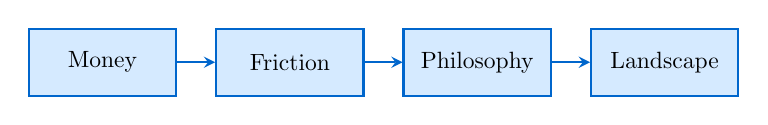
\begin{tikzpicture}[node distance=2.8cm, scale=0.85, transform shape]
\node (money) [process, minimum width=2.2cm] {Money};
\node (friction) [process, right of=money, minimum width=2.2cm] {Friction};
\node (philosophy) [process, right of=friction, minimum width=2.2cm] {Philosophy};
\node (landscape) [process, right of=philosophy, minimum width=2.2cm] {Landscape};
\draw [arrow] (money) -- (friction);
\draw [arrow] (friction) -- (philosophy);
\draw [arrow] (philosophy) -- (landscape);
\end{tikzpicture}
\end{center}
\end{frame}

% =====================================================================
% SECTION 1.1: WHAT IS MONEY, REALLY?
% =====================================================================
\section{1.1 What Is Money, Really?}

\begin{frame}{Topic 1.1: What Is Money, Really?}
\begin{center}
\textbf{\Large Trust, Ledgers, and the Problem of Double-Spending}
\end{center}

\vspace{5mm}
\textbf{Learning Objectives:}
\begin{itemize}
\item Dissolve assumptions about what money ``is''
\item Understand why digital money is fundamentally hard
\item Grasp the double-spending problem
\item Distinguish account-based from token-based money
\end{itemize}

\vspace{5mm}
\begin{block}{Hands-On Component}
We'll use a Colab notebook to simulate a simple ledger and see double-spending in action.
\end{block}
\end{frame}

\begin{frame}{A Thought Experiment}
\begin{center}
\textbf{\Large Imagine you're stranded on an island with 9 strangers...}
\end{center}

\vspace{5mm}
\begin{columns}[T]
\begin{column}{0.5\textwidth}
\textbf{You have skills:}
\begin{itemize}
\item Alice: fishing
\item Bob: building
\item Carol: farming
\item Dave: medicine
\item ...and so on
\end{itemize}
\end{column}
\begin{column}{0.5\textwidth}
\textbf{The problem:}
\begin{itemize}
\item Alice wants vegetables
\item Carol doesn't need fish
\item How do you trade?
\end{itemize}
\end{column}
\end{columns}

\vspace{5mm}
\begin{alertblock}{The Coincidence of Wants Problem}
Direct barter requires both parties to want what the other has, at the same time. This almost never happens.
\end{alertblock}
\end{frame}

\begin{frame}{Three Solutions to the Barter Problem}
\begin{center}
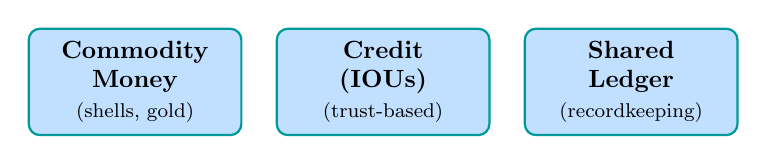
\begin{tikzpicture}[node distance=3.5cm, scale=0.9, transform shape]
% Solution 1: Commodity Money
\node (commodity) [blockchain, minimum width=3cm, minimum height=1.5cm] {
\begin{tabular}{c}
\textbf{Commodity}\\
\textbf{Money}\\
\footnotesize (shells, gold)
\end{tabular}
};

% Solution 2: Credit/Debt
\node (credit) [blockchain, right of=commodity, minimum width=3cm, minimum height=1.5cm] {
\begin{tabular}{c}
\textbf{Credit}\\
\textbf{(IOUs)}\\
\footnotesize (trust-based)
\end{tabular}
};

% Solution 3: Ledger
\node (ledger) [blockchain, right of=credit, minimum width=3cm, minimum height=1.5cm] {
\begin{tabular}{c}
\textbf{Shared}\\
\textbf{Ledger}\\
\footnotesize (recordkeeping)
\end{tabular}
};

\end{tikzpicture}
\end{center}

\vspace{5mm}
\textbf{Key Insight:} All three solutions are really about \textcolor{dfblue}{\textbf{trust}}.
\begin{itemize}
\item Commodity: Trust the material has value
\item Credit: Trust the person will repay
\item Ledger: Trust the recordkeeper is honest
\end{itemize}
\end{frame}

\begin{frame}{Money as a Social Technology}
\begin{columns}[T]
\begin{column}{0.55\textwidth}
\textbf{The Three Functions of Money:}
\begin{enumerate}
\item \textbf{Medium of Exchange}\\
\footnotesize Accepted for transactions
\item \textbf{Unit of Account}\\
\footnotesize Common measure of value
\item \textbf{Store of Value}\\
\footnotesize Holds purchasing power over time
\end{enumerate}

\vspace{3mm}
\textbf{What makes something ``money''?}\\
\textcolor{dfteal}{Collective belief that others will accept it.}
\end{column}
\begin{column}{0.42\textwidth}
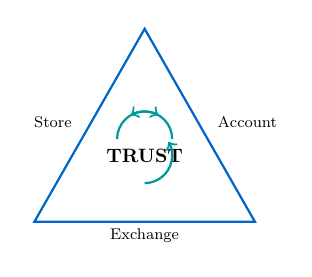
\begin{tikzpicture}[scale=0.7, transform shape]
% Triangle of money functions
\coordinate (A) at (0,0);
\coordinate (B) at (4,0);
\coordinate (C) at (2,3.5);

\draw[thick, dfblue] (A) -- (B) -- (C) -- cycle;

\node at (2,1.2) {\textbf{TRUST}};
\node[below] at (2,0) {\footnotesize Exchange};
\node[left] at (0.8,1.8) {\footnotesize Store};
\node[right] at (3.2,1.8) {\footnotesize Account};

% Add circular arrows suggesting interconnection
\draw[->, dfteal, thick] (1.5,1.5) arc (180:60:0.5);
\draw[->, dfteal, thick] (2.5,1.5) arc (0:120:0.5);
\draw[->, dfteal, thick] (2,0.7) arc (-90:30:0.5);
\end{tikzpicture}
\end{column}
\end{columns}

\vspace{3mm}
\begin{block}{Anthropological Fact}
Debt and credit systems (ledgers) predate physical currency by thousands of years. Money is fundamentally about \textbf{information}, not objects.
\end{block}
\end{frame}

\begin{frame}{The Ledger: Humanity's Oldest Financial Technology}
\begin{center}
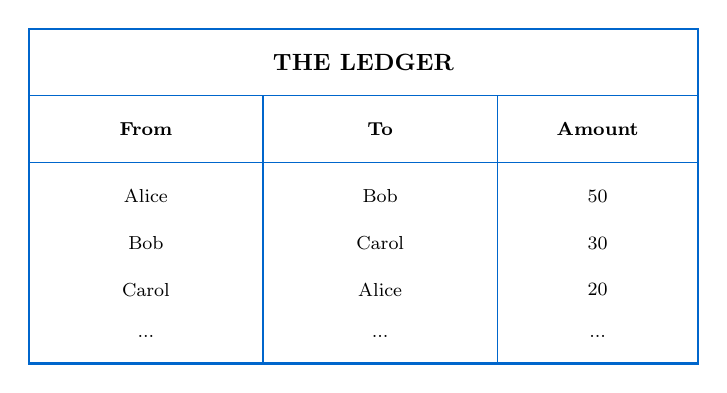
\begin{tikzpicture}[scale=0.85, transform shape]
% Simple ledger representation
\draw[thick, dfblue] (0,0) rectangle (10,5);
\node at (5,4.5) {\textbf{THE LEDGER}};
\draw[dfblue] (0,4) -- (10,4);

% Header
\draw[dfblue] (3.5,4) -- (3.5,0);
\draw[dfblue] (7,4) -- (7,0);
\node at (1.75,3.5) {\footnotesize \textbf{From}};
\node at (5.25,3.5) {\footnotesize \textbf{To}};
\node at (8.5,3.5) {\footnotesize \textbf{Amount}};
\draw[dfblue] (0,3) -- (10,3);

% Transactions
\node at (1.75,2.5) {\footnotesize Alice};
\node at (5.25,2.5) {\footnotesize Bob};
\node at (8.5,2.5) {\footnotesize 50};

\node at (1.75,1.8) {\footnotesize Bob};
\node at (5.25,1.8) {\footnotesize Carol};
\node at (8.5,1.8) {\footnotesize 30};

\node at (1.75,1.1) {\footnotesize Carol};
\node at (5.25,1.1) {\footnotesize Alice};
\node at (8.5,1.1) {\footnotesize 20};

\node at (1.75,0.4) {\footnotesize ...};
\node at (5.25,0.4) {\footnotesize ...};
\node at (8.5,0.4) {\footnotesize ...};
\end{tikzpicture}
\end{center}

\vspace{3mm}
\textbf{A ledger is simply:} A record of who owes what to whom.

\textbf{The critical question:} \textcolor{dfred}{Who maintains the ledger?}
\end{frame}

\begin{frame}{Account-Based vs. Token-Based Money}
\begin{columns}[T]
\begin{column}{0.48\textwidth}
\begin{block}{Account-Based (Ledger)}
\begin{center}
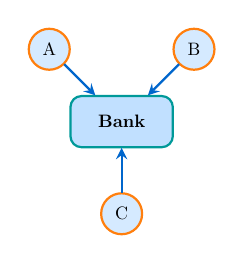
\begin{tikzpicture}[scale=0.65, transform shape]
% Central ledger
\node (bank) [blockchain, minimum width=2cm] {\textbf{Bank}};
\node (alice) [transaction, above left of=bank, node distance=2cm] {A};
\node (bob) [transaction, above right of=bank, node distance=2cm] {B};
\node (carol) [transaction, below of=bank, node distance=1.8cm] {C};

\draw[arrow] (alice) -- (bank);
\draw[arrow] (bob) -- (bank);
\draw[arrow] (carol) -- (bank);
\end{tikzpicture}
\end{center}
\begin{itemize}\compactlist
\item Identity verified
\item Balances in database
\item Transfers update records
\item \textbf{Example:} Bank accounts
\end{itemize}
\end{block}
\end{column}
\begin{column}{0.48\textwidth}
\begin{block}{Token-Based (Bearer)}
\begin{center}
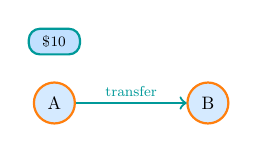
\begin{tikzpicture}[scale=0.65, transform shape]
% Direct transfer
\node (alice) [transaction] {A};
\node (bob) [transaction, right of=alice, node distance=3cm] {B};
\node (token) [blockchain, above of=alice, node distance=1.2cm, minimum width=1cm, minimum height=0.5cm] {\footnotesize \$10};

\draw[->, thick, dfteal] (alice) -- node[above] {\footnotesize transfer} (bob);
\end{tikzpicture}
\end{center}
\begin{itemize}\compactlist
\item Possession = ownership
\item No identity needed
\item Physical handoff
\item \textbf{Example:} Cash, gold
\end{itemize}
\end{block}
\end{column}
\end{columns}

\vspace{3mm}
\begin{alertblock}{The Digital Dilemma}
Physical tokens can be handed over. Digital files can be \textbf{copied}. How do you hand over a digital token without copying it?
\end{alertblock}
\end{frame}

\begin{frame}{The Double-Spending Problem}
\begin{center}
\textbf{\Large The Fundamental Challenge of Digital Money}
\end{center}

\begin{columns}[T]
\begin{column}{0.55\textwidth}
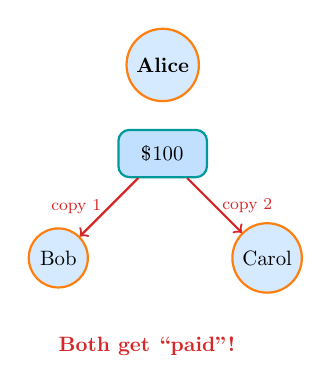
\begin{tikzpicture}[scale=0.75, transform shape, node distance=2cm]
% Alice with digital coin
\node (alice) [transaction, minimum size=1.2cm] {\textbf{Alice}};
\node (coin) [blockchain, below of=alice, minimum width=1.5cm, minimum height=0.8cm, node distance=1.5cm] {\$100};
\node (bob) [transaction, below left of=coin, minimum size=1cm, node distance=2.5cm] {Bob};
\node (carol) [transaction, below right of=coin, minimum size=1cm, node distance=2.5cm] {Carol};

% Arrows showing double spend
\draw[->, thick, dfred] (coin) -- node[left, font=\footnotesize] {copy 1} (bob);
\draw[->, thick, dfred] (coin) -- node[right, font=\footnotesize] {copy 2} (carol);

% Warning
\node[below of=bob, node distance=1.5cm, xshift=1.5cm] {\textcolor{dfred}{\textbf{Both get ``paid''!}}};
\end{tikzpicture}
\end{column}
\begin{column}{0.42\textwidth}
\textbf{Why is this hard?}
\begin{itemize}
\item Digital = perfectly copyable
\item No physical scarcity
\item Can't ``hand over'' a file
\item Need to prevent copies from both being valid
\end{itemize}

\vspace{3mm}
\textbf{Before 2008, only one solution existed:}\\
\textcolor{dfteal}{A trusted central authority}
\end{column}
\end{columns}
\end{frame}

\begin{frame}{The Traditional Solution: Trusted Third Parties}
\begin{center}
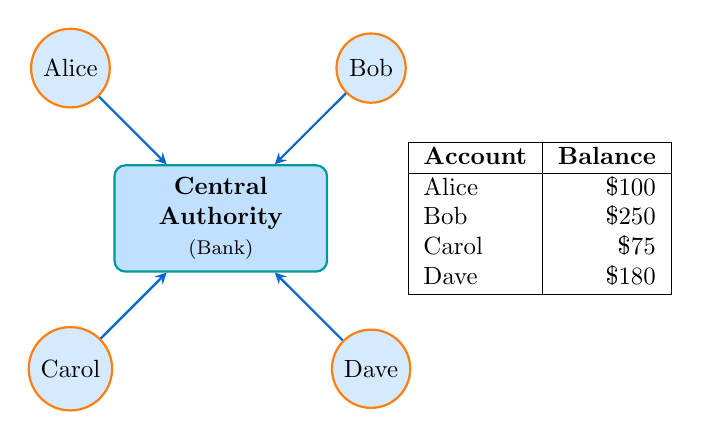
\begin{tikzpicture}[scale=0.9, transform shape]
% Central authority
\node (bank) [blockchain, minimum width=3cm, minimum height=1.5cm] {
\begin{tabular}{c}
\textbf{Central}\\
\textbf{Authority}\\
\footnotesize (Bank)
\end{tabular}
};

% Users around
\node (alice) [transaction, above left of=bank, node distance=3cm] {Alice};
\node (bob) [transaction, above right of=bank, node distance=3cm] {Bob};
\node (carol) [transaction, below left of=bank, node distance=3cm] {Carol};
\node (dave) [transaction, below right of=bank, node distance=3cm] {Dave};

% Connections
\draw[arrow] (alice) -- (bank);
\draw[arrow] (bob) -- (bank);
\draw[arrow] (carol) -- (bank);
\draw[arrow] (dave) -- (bank);

% Ledger
\node[right of=bank, node distance=4.5cm] {
\begin{tabular}{|l|r|}
\hline
\textbf{Account} & \textbf{Balance} \\
\hline
Alice & \$100 \\
Bob & \$250 \\
Carol & \$75 \\
Dave & \$180 \\
\hline
\end{tabular}
};
\end{tikzpicture}
\end{center}

\textbf{How it prevents double-spending:}
\begin{enumerate}
\item Alice requests: ``Send \$100 to Bob''
\item Bank checks: Does Alice have \$100?
\item Bank updates: Alice $-$\$100, Bob $+$\$100
\item Transaction complete---Alice can't spend it again
\end{enumerate}
\end{frame}

\begin{frame}{The Cost of Trust}
\begin{columns}[T]
\begin{column}{0.48\textwidth}
\textbf{What we gain:}
\begin{itemize}
\item Double-spending prevented
\item Transaction records
\item Dispute resolution
\item Reversibility (chargebacks)
\end{itemize}

\vspace{5mm}
\textbf{What we lose:}
\begin{itemize}
\item Privacy (bank sees everything)
\item Autonomy (bank can freeze accounts)
\item Inclusion (need bank approval)
\item Speed (bank's hours, processes)
\item Cost (bank's fees)
\end{itemize}
\end{column}
\begin{column}{0.48\textwidth}
\begin{alertblock}{The Trust Assumption}
We must trust that the central authority:
\begin{itemize}\compactlist
\item Won't steal our money
\item Won't censor transactions
\item Won't fail or get hacked
\item Will always be available
\item Will treat everyone fairly
\end{itemize}
\end{alertblock}

\vspace{2mm}
\textbf{2008 Financial Crisis:}\\
\footnotesize Many questioned whether this trust was warranted.
\end{column}
\end{columns}
\end{frame}

\begin{frame}{The Bitcoin Breakthrough (Preview)}
\begin{center}
\textbf{\Large What if we could prevent double-spending \textit{without} a central authority?}
\end{center}

\vspace{3mm}
\begin{columns}[T]
\begin{column}{0.48\textwidth}
\textbf{Satoshi Nakamoto's insight:}
\begin{enumerate}
\item Replicate the ledger everywhere
\item Use cryptography to verify
\item Use economic incentives to secure
\item Achieve consensus without trust
\end{enumerate}
\end{column}
\begin{column}{0.48\textwidth}
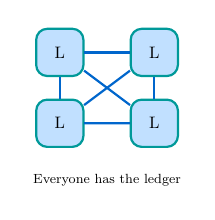
\begin{tikzpicture}[scale=0.6, transform shape]
% Distributed network
\node (n1) [blockchain, minimum width=1cm] {L};
\node (n2) [blockchain, right of=n1, node distance=2cm, minimum width=1cm] {L};
\node (n3) [blockchain, below of=n1, node distance=1.5cm, minimum width=1cm] {L};
\node (n4) [blockchain, below of=n2, node distance=1.5cm, minimum width=1cm] {L};

\draw[thick, dfblue] (n1) -- (n2);
\draw[thick, dfblue] (n1) -- (n3);
\draw[thick, dfblue] (n1) -- (n4);
\draw[thick, dfblue] (n2) -- (n3);
\draw[thick, dfblue] (n2) -- (n4);
\draw[thick, dfblue] (n3) -- (n4);

\node[below of=n3, node distance=1.2cm, xshift=1cm] {\footnotesize Everyone has the ledger};
\end{tikzpicture}
\end{column}
\end{columns}

\vspace{5mm}
\begin{block}{We'll Explore This in Day 3}
For now, understand that \textbf{blockchain} is one answer to: ``How do we have digital money without trusting a single party?''
\end{block}
\end{frame}

\begin{frame}{Hands-On: Ledger Simulation}
\begin{center}
\textbf{\Large Let's See Double-Spending in Action}
\end{center}

\vspace{5mm}
\textbf{In the Colab notebook, we will:}
\begin{enumerate}
\item Build a simple ledger with account balances
\item Process valid transactions
\item Attempt a double-spend attack
\item See how a central authority prevents it
\item Discuss: What happens without the authority?
\end{enumerate}

\vspace{5mm}
\begin{block}{Access the Notebook}
\texttt{day\_01/notebooks/01\_ledger\_simulation.ipynb}

\vspace{2mm}
\footnotesize Or scan QR code / click link provided
\end{block}

\bottomnote{Time: 15-20 minutes for guided exploration}
\end{frame}

\begin{frame}{Discussion: Money in the Digital Age}
\begin{columns}[T]
\begin{column}{0.48\textwidth}
\textbf{Questions to Consider:}
\begin{enumerate}
\item Is Bitcoin ``real money''? Why or why not?
\item What makes you trust your bank?
\item If you could design money from scratch, what would it look like?
\item Is privacy a feature or a bug?
\end{enumerate}
\end{column}
\begin{column}{0.48\textwidth}
\textbf{Key Takeaways:}
\begin{itemize}
\item Money = trust infrastructure
\item Digital money needs double-spend protection
\item Central authorities work but have costs
\item Blockchain offers an alternative
\end{itemize}
\end{column}
\end{columns}

\vspace{5mm}
\begin{alertblock}{The Central Question of This Course}
How should we build the trust infrastructure for a digital economy?
\end{alertblock}
\end{frame}

% =====================================================================
% SECTION 1.2: THE FINANCIAL SYSTEM'S PAIN POINTS
% =====================================================================
\section{1.2 Financial System's Pain Points}

\begin{frame}{Topic 1.2: The Financial System's Pain Points}
\begin{center}
\textbf{\Large Where Friction Creates Opportunity}
\end{center}

\vspace{5mm}
\textbf{Learning Objectives:}
\begin{itemize}
\item Identify 4-5 core frictions in traditional finance
\item Understand who bears the cost of each friction
\item See friction as the \textit{motivation} for digital finance innovation
\end{itemize}

\vspace{5mm}
\begin{block}{Why This Matters}
Every FinTech and DeFi innovation targets a specific friction. Understanding the frictions helps you understand the solutions.
\end{block}
\end{frame}

\begin{frame}{The Global Financial System: A Marvel of Complexity}
\begin{center}
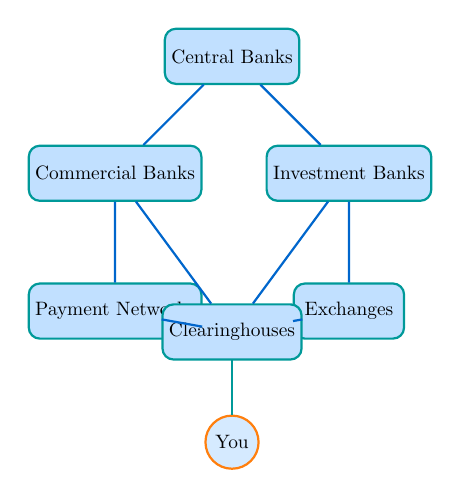
\begin{tikzpicture}[scale=0.7, transform shape]
% Central banks
\node (fed) [blockchain, minimum width=2cm] {Central Banks};
\node (comm) [blockchain, below left of=fed, node distance=3cm, minimum width=2cm] {Commercial Banks};
\node (inv) [blockchain, below right of=fed, node distance=3cm, minimum width=2cm] {Investment Banks};
\node (pay) [blockchain, below of=comm, node distance=2.5cm, minimum width=2cm] {Payment Networks};
\node (exch) [blockchain, below of=inv, node distance=2.5cm, minimum width=2cm] {Exchanges};
\node (clear) [blockchain, below of=fed, node distance=5cm, minimum width=2cm] {Clearinghouses};

% Connections
\draw[thick, dfblue] (fed) -- (comm);
\draw[thick, dfblue] (fed) -- (inv);
\draw[thick, dfblue] (comm) -- (pay);
\draw[thick, dfblue] (inv) -- (exch);
\draw[thick, dfblue] (comm) -- (clear);
\draw[thick, dfblue] (inv) -- (clear);
\draw[thick, dfblue] (pay) -- (clear);
\draw[thick, dfblue] (exch) -- (clear);

% Users
\node (user) [transaction, below of=clear, node distance=2cm] {You};
\draw[thick, dfteal] (user) -- (clear);
\end{tikzpicture}
\end{center}

\footnotesize
This system moves \textbf{\$9.6 trillion daily}, serves billions, rarely fails catastrophically... but has significant frictions.
\end{frame}

\begin{frame}{Friction \#1: Slow Settlement}
\begin{columns}[T]
\begin{column}{0.55\textwidth}
\textbf{The Problem:}
\begin{itemize}
\item Stock trade: T+1 (1 business day to settle since May 2024)
\item International wire: 1-5 business days
\item ACH transfer: 2-3 business days
\item Even ``instant'' payments take hours behind scenes
\end{itemize}

\vspace{3mm}
\textbf{Why so slow?}
\begin{itemize}
\item Multiple intermediaries
\item Batch processing (not real-time)
\item Timezone differences
\item Manual compliance checks
\item Legacy systems from 1970s
\end{itemize}
\end{column}
\begin{column}{0.42\textwidth}
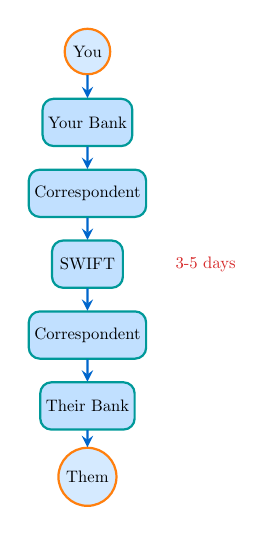
\begin{tikzpicture}[scale=0.6, transform shape, node distance=1.5cm]
% Settlement chain
\node (you) [transaction] {You};
\node (bank1) [blockchain, below of=you, minimum width=1.5cm] {Your Bank};
\node (corr1) [blockchain, below of=bank1, minimum width=1.5cm] {Correspondent};
\node (swift) [blockchain, below of=corr1, minimum width=1.5cm] {SWIFT};
\node (corr2) [blockchain, below of=swift, minimum width=1.5cm] {Correspondent};
\node (bank2) [blockchain, below of=corr2, minimum width=1.5cm] {Their Bank};
\node (them) [transaction, below of=bank2] {Them};

\draw[arrow] (you) -- (bank1);
\draw[arrow] (bank1) -- (corr1);
\draw[arrow] (corr1) -- (swift);
\draw[arrow] (swift) -- (corr2);
\draw[arrow] (corr2) -- (bank2);
\draw[arrow] (bank2) -- (them);

\node[right of=swift, node distance=2.5cm] {\textcolor{dfred}{3-5 days}};
\end{tikzpicture}
\end{column}
\end{columns}
\end{frame}

\begin{frame}{Friction \#2: High Fees (Especially Cross-Border)}
\begin{center}
\textbf{Cost of Sending \$200 Internationally}
\end{center}

\begin{center}
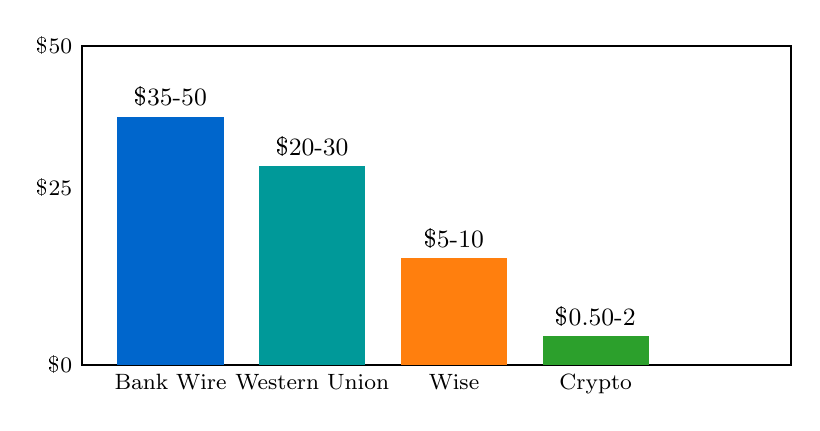
\begin{tikzpicture}[scale=0.9]
% Bar chart
\draw[thick] (0,0) -- (10,0) -- (10,4.5) -- (0,4.5) -- cycle;

% Bars
\fill[dfblue] (0.5,0) rectangle (2,3.5);
\fill[dfteal] (2.5,0) rectangle (4,2.8);
\fill[dforange] (4.5,0) rectangle (6,1.5);
\fill[dfgreen] (6.5,0) rectangle (8,0.4);

% Labels
\node[below, font=\footnotesize] at (1.25,0) {Bank Wire};
\node[below, font=\footnotesize] at (3.25,0) {Western Union};
\node[below, font=\footnotesize] at (5.25,0) {Wise};
\node[below, font=\footnotesize] at (7.25,0) {Crypto};

% Values
\node[above, font=\small] at (1.25,3.5) {\$35-50};
\node[above, font=\small] at (3.25,2.8) {\$20-30};
\node[above, font=\small] at (5.25,1.5) {\$5-10};
\node[above, font=\small] at (7.25,0.4) {\$0.50-2};

% Y-axis
\node[left] at (0,0) {\footnotesize \$0};
\node[left] at (0,2.5) {\footnotesize \$25};
\node[left] at (0,4.5) {\footnotesize \$50};
\end{tikzpicture}
\end{center}

\vspace{3mm}
\textbf{Who pays?} Migrant workers sending money home. The global remittance market is \textbf{\$700+ billion/year}, with \textbf{\$50+ billion} lost to fees.
\end{frame}

\begin{frame}{Friction \#3: Financial Exclusion}
\begin{columns}[T]
\begin{column}{0.5\textwidth}
\textbf{The Unbanked and Underbanked:}
\begin{itemize}
\item \textbf{1.4 billion} adults globally have no bank account
\item \textbf{Additional 1+ billion} are underbanked
\item In the US: 6\% unbanked, 18\% underbanked
\end{itemize}

\vspace{3mm}
\textbf{Why excluded?}
\begin{itemize}
\item No ID documents
\item No fixed address
\item Minimum balance requirements
\item Poor credit history
\item Geographic distance from banks
\item Distrust of institutions
\end{itemize}
\end{column}
\begin{column}{0.48\textwidth}
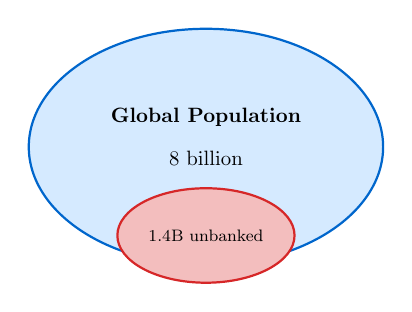
\begin{tikzpicture}[scale=0.75, transform shape]
% World map representation (simplified)
\draw[thick, dfblue, fill=dflightblue4] (0,0) ellipse (3cm and 2cm);
\node at (0,0.5) {\textbf{Global Population}};
\node at (0,-0.2) {8 billion};

% Excluded portion
\draw[thick, dfred, fill=dfred!30] (0,-1.5) ellipse (1.5cm and 0.8cm);
\node[font=\footnotesize] at (0,-1.5) {1.4B unbanked};
\end{tikzpicture}

\vspace{3mm}
\begin{alertblock}{The Paradox}
Those who need financial services most have the least access to them.
\end{alertblock}
\end{column}
\end{columns}
\end{frame}

\begin{frame}{Friction \#4: Opacity and Information Asymmetry}
\begin{columns}[T]
\begin{column}{0.55\textwidth}
\textbf{What you don't know:}
\begin{itemize}
\item True cost of financial products
\item Where your money goes
\item How prices are determined
\item What risks you're taking
\item How algorithms affect you
\end{itemize}

\vspace{3mm}
\textbf{Examples:}
\begin{itemize}
\item Hidden fees in mutual funds (expense ratios)
\item Payment for order flow in stock trading
\item Credit card interchange fees
\item Insurance pricing algorithms
\end{itemize}
\end{column}
\begin{column}{0.42\textwidth}
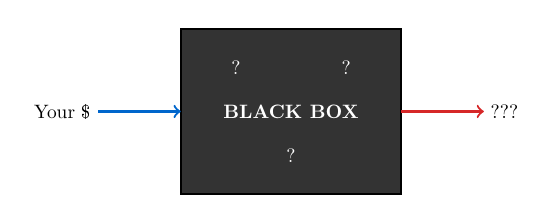
\begin{tikzpicture}[scale=0.7, transform shape]
% Black box
\draw[thick, fill=black!80] (0,0) rectangle (4,3);
\node[white] at (2,1.5) {\textbf{BLACK BOX}};

% Input
\draw[->, thick, dfblue] (-1.5,1.5) -- (0,1.5);
\node[left] at (-1.5,1.5) {Your \$};

% Output
\draw[->, thick, dfred] (4,1.5) -- (5.5,1.5);
\node[right] at (5.5,1.5) {???};

% Question marks
\node[white] at (1,2.3) {?};
\node[white] at (2,0.7) {?};
\node[white] at (3,2.3) {?};
\end{tikzpicture}

\vspace{5mm}
\footnotesize
\textbf{Information asymmetry} = one party knows more than the other. Usually favors financial institutions.
\end{column}
\end{columns}
\end{frame}

\begin{frame}{Friction \#5: Fragmentation and Incompatibility}
\begin{center}
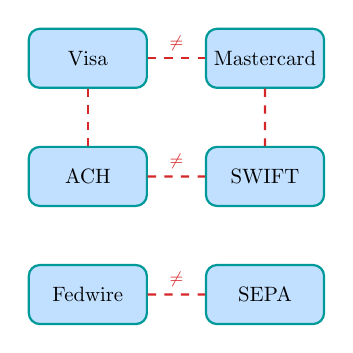
\begin{tikzpicture}[scale=0.75, transform shape]
% Different systems
\node (visa) [blockchain, minimum width=2cm] {Visa};
\node (mc) [blockchain, right of=visa, node distance=3cm, minimum width=2cm] {Mastercard};
\node (ach) [blockchain, below of=visa, node distance=2cm, minimum width=2cm] {ACH};
\node (swift) [blockchain, below of=mc, node distance=2cm, minimum width=2cm] {SWIFT};
\node (fed) [blockchain, below of=ach, node distance=2cm, minimum width=2cm] {Fedwire};
\node (sepa) [blockchain, below of=swift, node distance=2cm, minimum width=2cm] {SEPA};

% Show incompatibility
\draw[thick, dfred, dashed] (visa) -- node[above, font=\footnotesize] {$\neq$} (mc);
\draw[thick, dfred, dashed] (ach) -- node[above, font=\footnotesize] {$\neq$} (swift);
\draw[thick, dfred, dashed] (fed) -- node[above, font=\footnotesize] {$\neq$} (sepa);
\draw[thick, dfred, dashed] (visa) -- (ach);
\draw[thick, dfred, dashed] (mc) -- (swift);
\end{tikzpicture}
\end{center}

\textbf{The result:}
\begin{itemize}
\item Moving money between systems is expensive
\item Data doesn't flow smoothly
\item Innovation is slow (must work with legacy systems)
\item Lock-in effects (hard to switch providers)
\end{itemize}
\end{frame}

\begin{frame}{Friction \#6: Limited Operating Hours}
\begin{center}
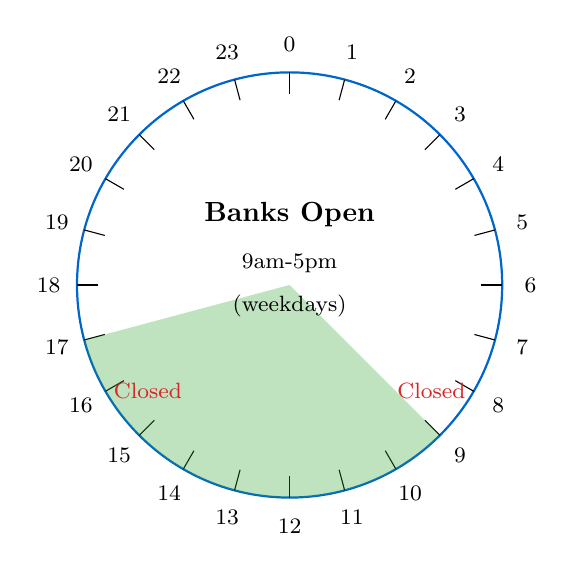
\begin{tikzpicture}[scale=0.9]
% 24-hour clock
\draw[thick, dfblue] (0,0) circle (3cm);

% Hours
\foreach \i in {0,1,...,23} {
    \draw ({90-\i*15}:2.7) -- ({90-\i*15}:3);
    \node at ({90-\i*15}:3.4) {\footnotesize \i};
}

% Business hours (shaded)
\fill[dfgreen, opacity=0.3] (0,0) -- (90-9*15:3) arc (90-9*15:90-17*15:3) -- cycle;

% Labels
\node at (0,1) {\textbf{Banks Open}};
\node at (0,0.3) {\footnotesize 9am-5pm};
\node at (0,-0.3) {\footnotesize (weekdays)};

% Night hours
\node[dfred] at (-2,-1.5) {\footnotesize Closed};
\node[dfred] at (2,-1.5) {\footnotesize Closed};
\end{tikzpicture}
\end{center}

\vspace{3mm}
\textbf{Traditional finance operates on:}
\begin{itemize}
\item Business hours only (no nights, weekends, holidays)
\item Local timezone (misaligned with global commerce)
\item Batch processing cycles (not real-time)
\end{itemize}
\end{frame}

\begin{frame}{Who Bears the Cost?}
\begin{center}
\renewcommand{\arraystretch}{1.4}
\begin{tabular}{|l|l|p{5cm}|}
\hline
\textbf{Friction} & \textbf{Primary Cost Bearer} & \textbf{Impact} \\
\hline
Slow settlement & Businesses, traders & Tied-up capital, missed opportunities \\
\hline
High fees & Consumers, migrants & Reduced purchasing power \\
\hline
Exclusion & Poor, rural, undocumented & No access to savings, credit, insurance \\
\hline
Opacity & Retail investors & Worse outcomes, exploitation \\
\hline
Fragmentation & Everyone & Inefficiency, higher costs \\
\hline
Limited hours & Global businesses & Delays, cash flow problems \\
\hline
\end{tabular}
\end{center}

\vspace{3mm}
\begin{alertblock}{Key Insight}
Friction costs are \textbf{regressive}---they hurt those with less money more than those with more.
\end{alertblock}
\end{frame}

\begin{frame}{Friction as Opportunity}
\begin{center}
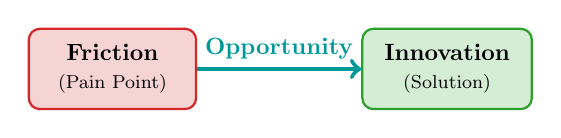
\begin{tikzpicture}[scale=0.85, transform shape, node distance=3cm]
% Friction to Innovation
\node (friction) [blockchain, minimum width=2.5cm, minimum height=1.2cm, fill=dfred!20, draw=dfred] {
\begin{tabular}{c}
\textbf{Friction}\\
\footnotesize (Pain Point)
\end{tabular}
};

\node (innovation) [blockchain, right of=friction, node distance=5cm, minimum width=2.5cm, minimum height=1.2cm, fill=dfgreen!20, draw=dfgreen] {
\begin{tabular}{c}
\textbf{Innovation}\\
\footnotesize (Solution)
\end{tabular}
};

\draw[->, ultra thick, dfteal] (friction) -- node[above] {\textbf{Opportunity}} (innovation);
\end{tikzpicture}
\end{center}

\vspace{3mm}
\begin{columns}[T]
\begin{column}{0.48\textwidth}
\textbf{Slow settlement} $\rightarrow$\\
\footnotesize Real-time payments, instant settlement

\textbf{High fees} $\rightarrow$\\
\footnotesize Low-cost transfers, crypto rails

\textbf{Exclusion} $\rightarrow$\\
\footnotesize Mobile money, neobanks
\end{column}
\begin{column}{0.48\textwidth}
\textbf{Opacity} $\rightarrow$\\
\footnotesize Transparent protocols, open data

\textbf{Fragmentation} $\rightarrow$\\
\footnotesize APIs, interoperability standards

\textbf{Limited hours} $\rightarrow$\\
\footnotesize 24/7 digital infrastructure
\end{column}
\end{columns}
\end{frame}

\begin{frame}{Discussion: Frictions You've Experienced}
\textbf{Think-Pair-Share:}
\begin{enumerate}
\item \textbf{Think} (2 min): Have you personally experienced any of these frictions?
\begin{itemize}
\item Waiting for a transfer?
\item Paying unexpected fees?
\item Difficulty opening an account?
\item Not understanding financial products?
\end{itemize}
\item \textbf{Pair} (3 min): Share your experience with a neighbor
\item \textbf{Share}: What patterns emerge?
\end{enumerate}

\vspace{5mm}
\begin{block}{Discussion Questions}
\begin{itemize}
\item Which friction affects you most?
\item Which friction causes the most societal harm?
\item Are any of these frictions \textit{features} rather than bugs?
\end{itemize}
\end{block}
\end{frame}

% =====================================================================
% SECTION 1.3: TWO PHILOSOPHIES -- FINTECH VS. CRYPTO/DEFI
% =====================================================================
\section{1.3 Two Philosophies: FinTech vs. Crypto/DeFi}

\begin{frame}{Topic 1.3: Two Philosophies of Change}
\begin{center}
\textbf{\Large FinTech vs. Crypto/DeFi}
\end{center}

\vspace{5mm}
\textbf{Learning Objectives:}
\begin{itemize}
\item Understand the fundamental difference between two approaches
\item Classify innovations as FinTech or Crypto/DeFi
\item Articulate tradeoffs of each philosophy
\end{itemize}

\vspace{5mm}
\begin{block}{The Central Fork}
Both FinTech and Crypto/DeFi target the same frictions.\\
They differ fundamentally in \textbf{how} they approach the solution.
\end{block}
\end{frame}

\begin{frame}{The Fundamental Fork}
\begin{center}
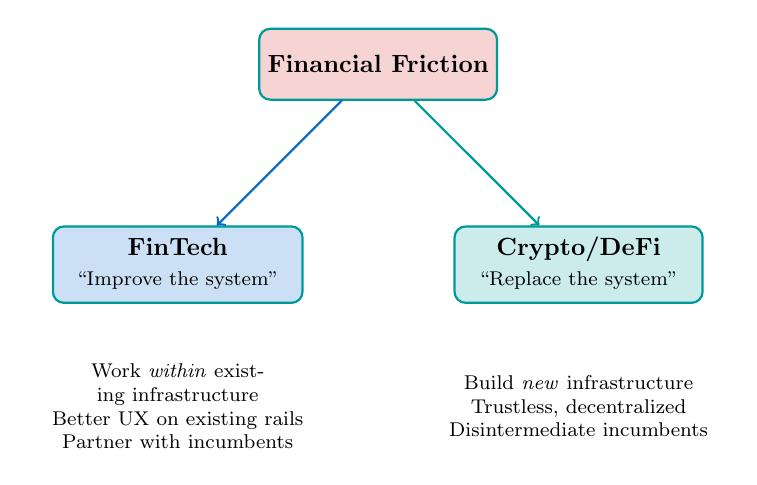
\begin{tikzpicture}[scale=0.9, transform shape]
% Root
\node (friction) [blockchain, minimum width=3cm, fill=dfred!20] {\textbf{Financial Friction}};

% Fork
\node (fintech) [blockchain, below left of=friction, node distance=4cm, minimum width=3.5cm, fill=dfblue!20] {
\begin{tabular}{c}
\textbf{FinTech}\\
\footnotesize ``Improve the system''
\end{tabular}
};

\node (crypto) [blockchain, below right of=friction, node distance=4cm, minimum width=3.5cm, fill=dfteal!20] {
\begin{tabular}{c}
\textbf{Crypto/DeFi}\\
\footnotesize ``Replace the system''
\end{tabular}
};

% Arrows
\draw[->, thick, dfblue] (friction) -- (fintech);
\draw[->, thick, dfteal] (friction) -- (crypto);

% Descriptions
\node[below of=fintech, node distance=2cm, text width=4cm, align=center, font=\footnotesize] {
Work \textit{within} existing infrastructure\\
Better UX on existing rails\\
Partner with incumbents
};

\node[below of=crypto, node distance=2cm, text width=4cm, align=center, font=\footnotesize] {
Build \textit{new} infrastructure\\
Trustless, decentralized\\
Disintermediate incumbents
};
\end{tikzpicture}
\end{center}
\end{frame}

\begin{frame}{Philosophy \#1: FinTech}
\begin{center}
\textbf{\Large ``Better UX on Existing Rails''}
\end{center}

\vspace{3mm}
\begin{columns}[T]
\begin{column}{0.5\textwidth}
\textbf{Core Belief:}\\
The existing financial infrastructure works. It just needs:
\begin{itemize}
\item Better user interfaces
\item More efficient processes
\item Smarter technology
\item New business models
\end{itemize}

\vspace{3mm}
\textbf{Key Technologies:}
\begin{itemize}
\item APIs and Open Banking
\item Mobile apps
\item Cloud computing
\item Machine learning
\item Big data analytics
\end{itemize}
\end{column}
\begin{column}{0.47\textwidth}
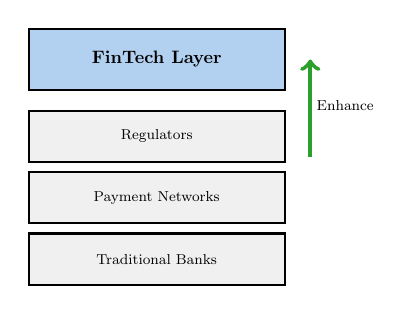
\begin{tikzpicture}[scale=0.65, transform shape]
% Traditional stack with FinTech layer
\draw[thick, fill=lightgray] (0,0) rectangle (5,1);
\node at (2.5,0.5) {\footnotesize Traditional Banks};

\draw[thick, fill=lightgray] (0,1.2) rectangle (5,2.2);
\node at (2.5,1.7) {\footnotesize Payment Networks};

\draw[thick, fill=lightgray] (0,2.4) rectangle (5,3.4);
\node at (2.5,2.9) {\footnotesize Regulators};

% FinTech layer on top
\draw[thick, fill=dfblue!30] (0,3.8) rectangle (5,5);
\node at (2.5,4.4) {\textbf{FinTech Layer}};

% Arrow showing enhancement
\draw[->, ultra thick, dfgreen] (5.5,2.5) -- (5.5,4.4);
\node[right, font=\footnotesize] at (5.5,3.5) {Enhance};
\end{tikzpicture}

\vspace{2mm}
\footnotesize
FinTech builds \textit{on top of} the existing system
\end{column}
\end{columns}
\end{frame}

\begin{frame}{FinTech Examples}
\begin{columns}[T]
\begin{column}{0.48\textwidth}
\textbf{Payments:}
\begin{itemize}
\item PayPal, Stripe, Square
\item Venmo, Cash App
\item Wise (TransferWise)
\end{itemize}

\vspace{3mm}
\textbf{Banking:}
\begin{itemize}
\item Chime, N26, Revolut
\item Nubank, Monzo
\item SoFi, Ally
\end{itemize}

\vspace{3mm}
\textbf{Lending:}
\begin{itemize}
\item LendingClub, Prosper
\item Affirm, Klarna (BNPL)
\item Upstart, Kabbage
\end{itemize}
\end{column}
\begin{column}{0.48\textwidth}
\textbf{Investing:}
\begin{itemize}
\item Robinhood, Webull
\item Betterment, Wealthfront
\item Acorns, Stash
\end{itemize}

\vspace{3mm}
\textbf{Insurance:}
\begin{itemize}
\item Lemonade, Oscar
\item Root, Hippo
\end{itemize}

\vspace{3mm}
\textbf{Common Thread:}\\
\textcolor{dfblue}{All use traditional rails (ACH, card networks, bank accounts) with better interfaces and processes.}
\end{column}
\end{columns}
\end{frame}

\begin{frame}{Philosophy \#2: Crypto/DeFi}
\begin{center}
\textbf{\Large ``New Rails, New Rules''}
\end{center}

\vspace{3mm}
\begin{columns}[T]
\begin{column}{0.5\textwidth}
\textbf{Core Belief:}\\
The existing infrastructure is fundamentally flawed. We need:
\begin{itemize}
\item New trust model (cryptographic, not institutional)
\item Decentralization (no single point of control)
\item Programmable money (smart contracts)
\item Permissionless access
\end{itemize}

\vspace{3mm}
\textbf{Key Technologies:}
\begin{itemize}
\item Blockchain and distributed ledgers
\item Public-key cryptography
\item Consensus mechanisms
\item Smart contracts
\end{itemize}
\end{column}
\begin{column}{0.47\textwidth}
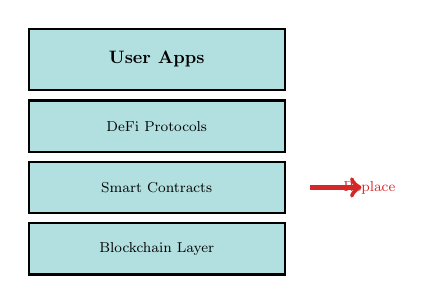
\begin{tikzpicture}[scale=0.65, transform shape]
% Traditional stack (grayed out)
\draw[thick, fill=lightgray, opacity=0.3] (0,0) rectangle (5,1);
\draw[thick, fill=lightgray, opacity=0.3] (0,1.2) rectangle (5,2.2);
\draw[thick, fill=lightgray, opacity=0.3] (0,2.4) rectangle (5,3.4);

% New stack
\draw[thick, fill=dfteal!30] (0,0) rectangle (5,1);
\node at (2.5,0.5) {\footnotesize Blockchain Layer};

\draw[thick, fill=dfteal!30] (0,1.2) rectangle (5,2.2);
\node at (2.5,1.7) {\footnotesize Smart Contracts};

\draw[thick, fill=dfteal!30] (0,2.4) rectangle (5,3.4);
\node at (2.5,2.9) {\footnotesize DeFi Protocols};

\draw[thick, fill=dfteal!30] (0,3.6) rectangle (5,4.8);
\node at (2.5,4.2) {\textbf{User Apps}};

% Arrow showing replacement
\draw[->, ultra thick, dfred] (5.5,1.7) -- node[right, font=\footnotesize] {Replace} (6.5,1.7);
\end{tikzpicture}

\vspace{2mm}
\footnotesize
Crypto/DeFi builds a \textit{parallel} system
\end{column}
\end{columns}
\end{frame}

\begin{frame}{Crypto/DeFi Examples}
\begin{columns}[T]
\begin{column}{0.48\textwidth}
\textbf{Currencies/Tokens:}
\begin{itemize}
\item Bitcoin, Ethereum
\item Stablecoins (USDC, USDT, DAI)
\item Layer 2s (Polygon, Arbitrum)
\end{itemize}

\vspace{3mm}
\textbf{Exchanges:}
\begin{itemize}
\item Uniswap, SushiSwap (DEX)
\item Coinbase, Binance (CEX bridges)
\item 0x, dYdX
\end{itemize}

\vspace{3mm}
\textbf{Lending:}
\begin{itemize}
\item Aave, Compound
\item MakerDAO
\item Liquity
\end{itemize}
\end{column}
\begin{column}{0.48\textwidth}
\textbf{Derivatives:}
\begin{itemize}
\item Synthetix
\item GMX, Perp Protocol
\end{itemize}

\vspace{3mm}
\textbf{Infrastructure:}
\begin{itemize}
\item Chainlink (oracles)
\item The Graph (indexing)
\item IPFS (storage)
\end{itemize}

\vspace{3mm}
\textbf{Common Thread:}\\
\textcolor{dfteal}{All operate on blockchain rails, using smart contracts, without traditional intermediaries.}
\end{column}
\end{columns}
\end{frame}

\begin{frame}{Side-by-Side Comparison}
\begin{center}
\renewcommand{\arraystretch}{1.3}
\begin{tabular}{|l|c|c|}
\hline
\textbf{Dimension} & \textbf{FinTech} & \textbf{Crypto/DeFi} \\
\hline
\textbf{Trust model} & Institutions & Code/Math \\
\hline
\textbf{Infrastructure} & Existing rails & New rails \\
\hline
\textbf{Permission} & Licensed, regulated & Permissionless \\
\hline
\textbf{Identity} & Required (KYC) & Optional (pseudonymous) \\
\hline
\textbf{Reversibility} & Chargebacks possible & Transactions final \\
\hline
\textbf{Speed to market} & Faster (use existing) & Slower (build new) \\
\hline
\textbf{Regulatory clarity} & Higher & Lower \\
\hline
\textbf{User experience} & Polished & Improving \\
\hline
\textbf{Censorship resistance} & Low & High \\
\hline
\end{tabular}
\end{center}
\end{frame}

\begin{frame}{Tradeoffs: FinTech}
\begin{columns}[T]
\begin{column}{0.48\textwidth}
\textbf{Advantages:}
\begin{itemize}
\item[\textcolor{dfgreen}{\checkmark}] Familiar UX
\item[\textcolor{dfgreen}{\checkmark}] Regulatory compliance
\item[\textcolor{dfgreen}{\checkmark}] Consumer protections
\item[\textcolor{dfgreen}{\checkmark}] Fiat integration
\item[\textcolor{dfgreen}{\checkmark}] Customer support
\item[\textcolor{dfgreen}{\checkmark}] Fast iteration
\item[\textcolor{dfgreen}{\checkmark}] Proven business models
\end{itemize}
\end{column}
\begin{column}{0.48\textwidth}
\textbf{Disadvantages:}
\begin{itemize}
\item[\textcolor{dfred}{$\times$}] Still intermediated
\item[\textcolor{dfred}{$\times$}] Geographic restrictions
\item[\textcolor{dfred}{$\times$}] Can be censored/frozen
\item[\textcolor{dfred}{$\times$}] Limited innovation ceiling
\item[\textcolor{dfred}{$\times$}] Data centralization
\item[\textcolor{dfred}{$\times$}] Dependent on banks
\item[\textcolor{dfred}{$\times$}] Exclusion still possible
\end{itemize}
\end{column}
\end{columns}

\vspace{5mm}
\begin{block}{Best For}
Users who want \textbf{better} financial services within the existing system, with familiar protections and convenience.
\end{block}
\end{frame}

\begin{frame}{Tradeoffs: Crypto/DeFi}
\begin{columns}[T]
\begin{column}{0.48\textwidth}
\textbf{Advantages:}
\begin{itemize}
\item[\textcolor{dfgreen}{\checkmark}] Permissionless access
\item[\textcolor{dfgreen}{\checkmark}] Censorship resistant
\item[\textcolor{dfgreen}{\checkmark}] Transparent (open-source)
\item[\textcolor{dfgreen}{\checkmark}] Composable (``money legos'')
\item[\textcolor{dfgreen}{\checkmark}] 24/7 global operation
\item[\textcolor{dfgreen}{\checkmark}] Self-custody possible
\item[\textcolor{dfgreen}{\checkmark}] Programmable money
\end{itemize}
\end{column}
\begin{column}{0.48\textwidth}
\textbf{Disadvantages:}
\begin{itemize}
\item[\textcolor{dfred}{$\times$}] Complex UX
\item[\textcolor{dfred}{$\times$}] Regulatory uncertainty
\item[\textcolor{dfred}{$\times$}] No chargebacks
\item[\textcolor{dfred}{$\times$}] Smart contract risks
\item[\textcolor{dfred}{$\times$}] Volatility (non-stablecoins)
\item[\textcolor{dfred}{$\times$}] Scalability challenges
\item[\textcolor{dfred}{$\times$}] ``Code is law'' rigidity
\end{itemize}
\end{column}
\end{columns}

\vspace{5mm}
\begin{block}{Best For}
Users who need \textbf{different} financial infrastructure---global access, self-sovereignty, censorship resistance, or programmable finance.
\end{block}
\end{frame}

\begin{frame}{The Convergence}
\begin{center}
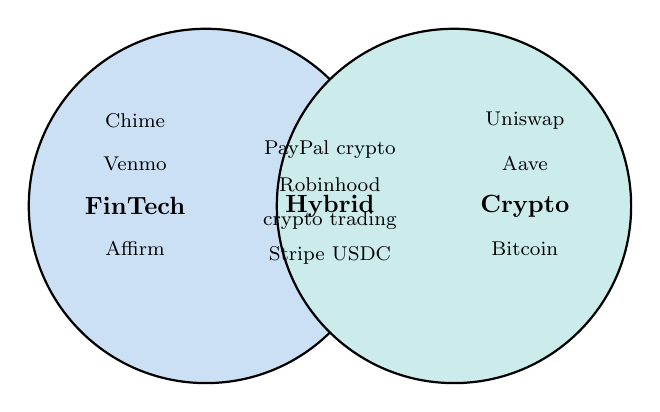
\begin{tikzpicture}[scale=0.9, transform shape]
% Two circles overlapping
\draw[thick, fill=dfblue!20] (0,0) circle (2.5cm);
\draw[thick, fill=dfteal!20] (3.5,0) circle (2.5cm);

% Labels
\node at (-1,0) {\textbf{FinTech}};
\node at (4.5,0) {\textbf{Crypto}};
\node at (1.75,0) {\textbf{Hybrid}};

% Examples in overlap
\node[font=\footnotesize] at (1.75,0.8) {PayPal crypto};
\node[font=\footnotesize] at (1.75,0.3) {Robinhood};
\node[font=\footnotesize] at (1.75,-0.2) {crypto trading};
\node[font=\footnotesize] at (1.75,-0.7) {Stripe USDC};

% Pure examples
\node[font=\footnotesize] at (-1,1.2) {Chime};
\node[font=\footnotesize] at (-1,0.6) {Venmo};
\node[font=\footnotesize] at (-1,-0.6) {Affirm};

\node[font=\footnotesize] at (4.5,1.2) {Uniswap};
\node[font=\footnotesize] at (4.5,0.6) {Aave};
\node[font=\footnotesize] at (4.5,-0.6) {Bitcoin};
\end{tikzpicture}
\end{center}

\vspace{3mm}
\textbf{Increasingly:}
\begin{itemize}
\item FinTech companies add crypto features
\item Crypto projects improve UX toward FinTech standards
\item Traditional banks explore blockchain
\item Lines blur, but philosophies remain distinct
\end{itemize}
\end{frame}

\begin{frame}{Classification Exercise}
\textbf{For each innovation, decide: FinTech or Crypto/DeFi?}

\vspace{3mm}
\begin{enumerate}
\item A mobile app that rounds up purchases and invests the change in ETFs
\pause
\textcolor{dfblue}{\textbf{FinTech}} (uses traditional brokerage)
\pause
\item A protocol that lets you earn interest by lending stablecoins
\pause
\textcolor{dfteal}{\textbf{Crypto/DeFi}} (smart contracts, no intermediary)
\pause
\item A bank that has no physical branches and only mobile apps
\pause
\textcolor{dfblue}{\textbf{FinTech}} (still a licensed bank, uses ACH)
\pause
\item A system where you can trade tokenized stocks 24/7
\pause
\textcolor{dfteal}{\textbf{Crypto/DeFi}} (synthetic assets, blockchain settlement)
\pause
\item A service that uses AI to approve loans faster
\pause
\textcolor{dfblue}{\textbf{FinTech}} (better process, same infrastructure)
\end{enumerate}
\end{frame}

\begin{frame}{Discussion: Which Philosophy Do You Prefer?}
\begin{columns}[T]
\begin{column}{0.48\textwidth}
\textbf{Team FinTech argues:}
\begin{itemize}
\item ``If it ain't broke, don't rebuild it''
\item Regulatory protection matters
\item Most users want convenience, not sovereignty
\item Crypto is too volatile and risky
\end{itemize}
\end{column}
\begin{column}{0.48\textwidth}
\textbf{Team Crypto argues:}
\begin{itemize}
\item ``The system IS broke for billions''
\item Financial freedom requires autonomy
\item Permissionless access is a human right
\item Code is more trustworthy than institutions
\end{itemize}
\end{column}
\end{columns}

\vspace{5mm}
\begin{block}{Discussion Questions}
\begin{itemize}
\item Is there room for both philosophies?
\item Under what circumstances would you choose each?
\item What would make you switch from one to the other?
\end{itemize}
\end{block}
\end{frame}

% =====================================================================
% SECTION 1.4: LANDSCAPE OVERVIEW
% =====================================================================
\section{1.4 Landscape Overview}

\begin{frame}{Topic 1.4: Landscape Overview}
\begin{center}
\textbf{\Large A Map of Digital Finance}
\end{center}

\vspace{5mm}
\textbf{Learning Objectives:}
\begin{itemize}
\item Visualize the full scope of digital finance
\item Understand how different sectors connect
\item Locate any innovation within the landscape
\end{itemize}

\vspace{5mm}
\begin{block}{Why a Map Matters}
Without structure, digital finance seems like ``a collection of cool things.''\\
A map lets you see patterns, gaps, and connections.
\end{block}
\end{frame}

\begin{frame}{The Digital Finance Landscape}
\begin{center}
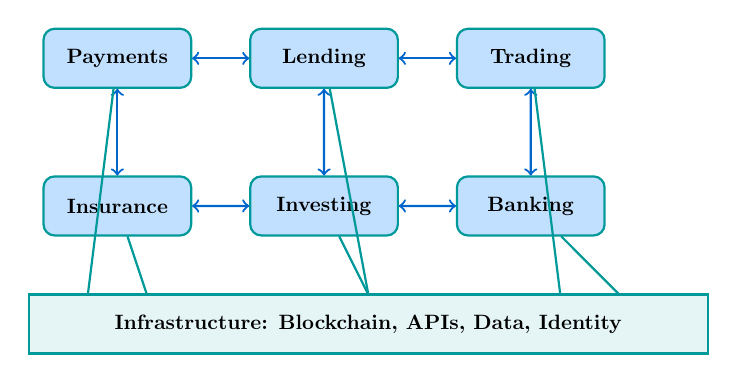
\begin{tikzpicture}[scale=0.75, transform shape]
% Main categories
\node (payments) [blockchain, minimum width=2.5cm, minimum height=1cm] {\textbf{Payments}};
\node (lending) [blockchain, right of=payments, node distance=3.5cm, minimum width=2.5cm, minimum height=1cm] {\textbf{Lending}};
\node (trading) [blockchain, right of=lending, node distance=3.5cm, minimum width=2.5cm, minimum height=1cm] {\textbf{Trading}};

\node (insurance) [blockchain, below of=payments, node distance=2.5cm, minimum width=2.5cm, minimum height=1cm] {\textbf{Insurance}};
\node (invest) [blockchain, below of=lending, node distance=2.5cm, minimum width=2.5cm, minimum height=1cm] {\textbf{Investing}};
\node (banking) [blockchain, below of=trading, node distance=2.5cm, minimum width=2.5cm, minimum height=1cm] {\textbf{Banking}};

% Infrastructure layer
\draw[thick, dfteal, fill=dfteal!10] (-1.5,-4) rectangle (10,-5);
\node at (4.25,-4.5) {\textbf{Infrastructure: Blockchain, APIs, Data, Identity}};

% Connections
\draw[thick, dfblue, <->] (payments) -- (lending);
\draw[thick, dfblue, <->] (lending) -- (trading);
\draw[thick, dfblue, <->] (payments) -- (insurance);
\draw[thick, dfblue, <->] (lending) -- (invest);
\draw[thick, dfblue, <->] (trading) -- (banking);
\draw[thick, dfblue, <->] (insurance) -- (invest);
\draw[thick, dfblue, <->] (invest) -- (banking);

% Connect to infrastructure
\draw[thick, dfteal] (payments) -- (-0.5,-4);
\draw[thick, dfteal] (insurance) -- (0.5,-4);
\draw[thick, dfteal] (lending) -- (4.25,-4);
\draw[thick, dfteal] (invest) -- (4.25,-4);
\draw[thick, dfteal] (trading) -- (7.5,-4);
\draw[thick, dfteal] (banking) -- (8.5,-4);
\end{tikzpicture}
\end{center}
\end{frame}

\begin{frame}{Sector 1: Payments}
\begin{columns}[T]
\begin{column}{0.48\textwidth}
\textbf{What it covers:}
\begin{itemize}
\item Person-to-person (P2P)
\item Consumer-to-business (C2B)
\item Business-to-business (B2B)
\item Cross-border remittances
\item Point-of-sale systems
\item Digital wallets
\end{itemize}

\vspace{3mm}
\textbf{Key friction addressed:}\\
Speed, cost, convenience
\end{column}
\begin{column}{0.48\textwidth}
\textbf{FinTech examples:}
\begin{itemize}
\item Venmo, Zelle, Cash App
\item Stripe, Square, Adyen
\item Wise, Remitly
\end{itemize}

\vspace{3mm}
\textbf{Crypto examples:}
\begin{itemize}
\item Bitcoin Lightning
\item USDC/USDT transfers
\item Solana Pay
\end{itemize}
\end{column}
\end{columns}

\vspace{3mm}
\begin{block}{Coming in Day 2}
Deep dive into payment infrastructure, rails, and the future of money movement.
\end{block}
\end{frame}

\begin{frame}{Sector 2: Lending}
\begin{columns}[T]
\begin{column}{0.48\textwidth}
\textbf{What it covers:}
\begin{itemize}
\item Consumer lending
\item SMB lending
\item Peer-to-peer lending
\item Buy-now-pay-later (BNPL)
\item Collateralized lending
\item Flash loans
\end{itemize}

\vspace{3mm}
\textbf{Key friction addressed:}\\
Access, speed, cost of credit
\end{column}
\begin{column}{0.48\textwidth}
\textbf{FinTech examples:}
\begin{itemize}
\item LendingClub, Upstart
\item Affirm, Klarna, Afterpay
\item Kabbage, Funding Circle
\end{itemize}

\vspace{3mm}
\textbf{Crypto examples:}
\begin{itemize}
\item Aave, Compound
\item MakerDAO (DAI)
\item Liquity, Euler
\end{itemize}
\end{column}
\end{columns}

\vspace{3mm}
\begin{block}{Coming in Days 2 \& 4}
Platform-based lending (Day 2), DeFi lending protocols (Day 4).
\end{block}
\end{frame}

\begin{frame}{Sector 3: Trading \& Exchanges}
\begin{columns}[T]
\begin{column}{0.48\textwidth}
\textbf{What it covers:}
\begin{itemize}
\item Stock trading
\item Crypto exchanges
\item Derivatives
\item Forex
\item NFT marketplaces
\item Tokenized assets
\end{itemize}

\vspace{3mm}
\textbf{Key friction addressed:}\\
Access, fees, transparency
\end{column}
\begin{column}{0.48\textwidth}
\textbf{FinTech examples:}
\begin{itemize}
\item Robinhood, Webull, eToro
\item Interactive Brokers
\item Public, Alpaca
\end{itemize}

\vspace{3mm}
\textbf{Crypto examples:}
\begin{itemize}
\item Uniswap, Curve, Balancer
\item dYdX, GMX
\item OpenSea, Blur
\end{itemize}
\end{column}
\end{columns}

\vspace{3mm}
\begin{block}{Coming in Days 3 \& 4}
Decentralized exchanges and AMMs (Days 3-4), trading mechanics.
\end{block}
\end{frame}

\begin{frame}{Sector 4: Investing \& Wealth Management}
\begin{columns}[T]
\begin{column}{0.48\textwidth}
\textbf{What it covers:}
\begin{itemize}
\item Robo-advisors
\item Fractional investing
\item Micro-investing
\item Alternative investments
\item Portfolio management
\item Yield aggregation
\end{itemize}

\vspace{3mm}
\textbf{Key friction addressed:}\\
Minimums, expertise, access
\end{column}
\begin{column}{0.48\textwidth}
\textbf{FinTech examples:}
\begin{itemize}
\item Betterment, Wealthfront
\item Acorns, Stash
\item Fundrise, Republic
\end{itemize}

\vspace{3mm}
\textbf{Crypto examples:}
\begin{itemize}
\item Yearn Finance
\item Index Coop
\item Enzyme Finance
\end{itemize}
\end{column}
\end{columns}

\vspace{3mm}
\begin{block}{Coming in Days 2 \& 4}
Robo-advisors and platform finance (Day 2), DeFi yield strategies (Day 4).
\end{block}
\end{frame}

\begin{frame}{Sector 5: Insurance}
\begin{columns}[T]
\begin{column}{0.48\textwidth}
\textbf{What it covers:}
\begin{itemize}
\item InsurTech platforms
\item Parametric insurance
\item Peer-to-peer insurance
\item Embedded insurance
\item Smart contract coverage
\end{itemize}

\vspace{3mm}
\textbf{Key friction addressed:}\\
Cost, claims, access, transparency
\end{column}
\begin{column}{0.48\textwidth}
\textbf{FinTech examples:}
\begin{itemize}
\item Lemonade, Root
\item Oscar, Hippo
\item Metromile
\end{itemize}

\vspace{3mm}
\textbf{Crypto examples:}
\begin{itemize}
\item Nexus Mutual
\item Cover Protocol
\item InsurAce
\end{itemize}
\end{column}
\end{columns}

\vspace{3mm}
\begin{block}{Coming in Day 5}
Insurance technology, parametric insurance, and DeFi coverage.
\end{block}
\end{frame}

\begin{frame}{Sector 6: Banking Infrastructure}
\begin{columns}[T]
\begin{column}{0.48\textwidth}
\textbf{What it covers:}
\begin{itemize}
\item Neobanks
\item Banking-as-a-Service (BaaS)
\item Core banking platforms
\item Open banking APIs
\item Account aggregation
\end{itemize}

\vspace{3mm}
\textbf{Key friction addressed:}\\
Fees, UX, bundling, access
\end{column}
\begin{column}{0.48\textwidth}
\textbf{FinTech examples:}
\begin{itemize}
\item Chime, N26, Revolut
\item Plaid, MX, Yodlee
\item Synapse, Unit, Treasury Prime
\end{itemize}

\vspace{3mm}
\textbf{Crypto parallels:}
\begin{itemize}
\item Self-custody wallets
\item Account abstraction (ERC-4337)
\item On-chain identity
\end{itemize}
\end{column}
\end{columns}

\vspace{3mm}
\begin{block}{Coming in Day 2}
Platform finance, open banking, and the future of banking infrastructure.
\end{block}
\end{frame}

\begin{frame}{Infrastructure Layer}
\begin{center}
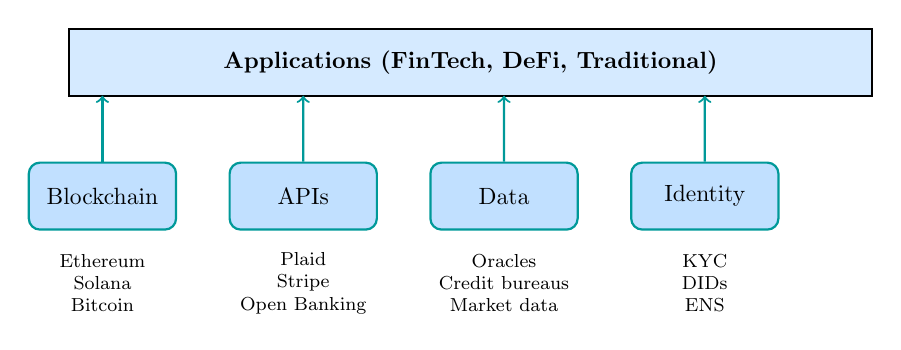
\begin{tikzpicture}[scale=0.85, transform shape]
% Infrastructure components
\node (blockchain) [blockchain, minimum width=2.2cm] {Blockchain};
\node (apis) [blockchain, right of=blockchain, node distance=3cm, minimum width=2.2cm] {APIs};
\node (data) [blockchain, right of=apis, node distance=3cm, minimum width=2.2cm] {Data};
\node (identity) [blockchain, right of=data, node distance=3cm, minimum width=2.2cm] {Identity};

% Applications layer above
\draw[thick, fill=dflightblue4] (-0.5,1.5) rectangle (11.5,2.5);
\node at (5.5,2) {\textbf{Applications (FinTech, DeFi, Traditional)}};

% Arrows up
\draw[->, thick, dfteal] (blockchain) -- ++(0,1.5);
\draw[->, thick, dfteal] (apis) -- ++(0,1.5);
\draw[->, thick, dfteal] (data) -- ++(0,1.5);
\draw[->, thick, dfteal] (identity) -- ++(0,1.5);

% Examples below each
\node[below of=blockchain, node distance=1.3cm, font=\footnotesize, text width=2cm, align=center] {Ethereum\\Solana\\Bitcoin};
\node[below of=apis, node distance=1.3cm, font=\footnotesize, text width=2cm, align=center] {Plaid\\Stripe\\Open Banking};
\node[below of=data, node distance=1.3cm, font=\footnotesize, text width=2cm, align=center] {Oracles\\Credit bureaus\\Market data};
\node[below of=identity, node distance=1.3cm, font=\footnotesize, text width=2cm, align=center] {KYC\\DIDs\\ENS};
\end{tikzpicture}
\end{center}

\vspace{3mm}
\textbf{Key insight:} All applications build on shared infrastructure.\\
Understanding the infrastructure helps you understand what's possible.
\end{frame}

\begin{frame}{Emerging Categories}
\begin{columns}[T]
\begin{column}{0.48\textwidth}
\textbf{Tokenization:}
\begin{itemize}
\item Real estate tokens
\item Art and collectibles
\item Carbon credits
\item Securities tokenization
\end{itemize}

\vspace{3mm}
\textbf{DAOs:}
\begin{itemize}
\item Decentralized governance
\item Treasury management
\item Collective investing
\end{itemize}
\end{column}
\begin{column}{0.48\textwidth}
\textbf{CBDCs:}
\begin{itemize}
\item Central Bank Digital Currencies
\item Government-issued digital money
\item Wholesale vs. retail
\end{itemize}

\vspace{3mm}
\textbf{AI + Finance:}
\begin{itemize}
\item Algorithmic credit scoring
\item Fraud detection
\item Automated advising
\item Predictive analytics
\end{itemize}
\end{column}
\end{columns}

\vspace{3mm}
\begin{block}{Coming in Days 5 \& 6}
Tokenization, DAOs, CBDCs, and the future of digital finance.
\end{block}
\end{frame}

\begin{frame}{Course Roadmap}
\begin{center}
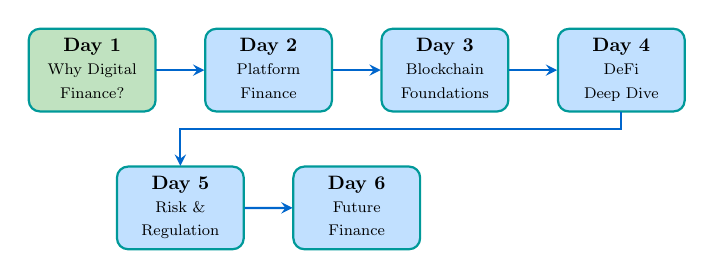
\begin{tikzpicture}[scale=0.7, transform shape]
% Days as nodes
\node (d1) [blockchain, minimum width=2.3cm, fill=dfgreen!30] {
\begin{tabular}{c}
\textbf{Day 1}\\
\footnotesize Why Digital\\
\footnotesize Finance?
\end{tabular}
};

\node (d2) [blockchain, right of=d1, node distance=3.2cm, minimum width=2.3cm] {
\begin{tabular}{c}
\textbf{Day 2}\\
\footnotesize Platform\\
\footnotesize Finance
\end{tabular}
};

\node (d3) [blockchain, right of=d2, node distance=3.2cm, minimum width=2.3cm] {
\begin{tabular}{c}
\textbf{Day 3}\\
\footnotesize Blockchain\\
\footnotesize Foundations
\end{tabular}
};

\node (d4) [blockchain, right of=d3, node distance=3.2cm, minimum width=2.3cm] {
\begin{tabular}{c}
\textbf{Day 4}\\
\footnotesize DeFi\\
\footnotesize Deep Dive
\end{tabular}
};

\node (d5) [blockchain, below of=d1, node distance=2.5cm, xshift=1.6cm, minimum width=2.3cm] {
\begin{tabular}{c}
\textbf{Day 5}\\
\footnotesize Risk \&\\
\footnotesize Regulation
\end{tabular}
};

\node (d6) [blockchain, right of=d5, node distance=3.2cm, minimum width=2.3cm] {
\begin{tabular}{c}
\textbf{Day 6}\\
\footnotesize Future\\
\footnotesize Finance
\end{tabular}
};

% Arrows
\draw[arrow] (d1) -- (d2);
\draw[arrow] (d2) -- (d3);
\draw[arrow] (d3) -- (d4);
\draw[arrow] (d4.south) -- ++(0,-0.3) -| (d5.north);
\draw[arrow] (d5) -- (d6);
\end{tikzpicture}
\end{center}

\textbf{You are here:} Day 1 -- building the foundation for everything that follows.
\end{frame}

\begin{frame}{Day 1 Synthesis}
\begin{columns}[T]
\begin{column}{0.48\textwidth}
\textbf{What We Covered:}
\begin{enumerate}
\item \textbf{Money} is trust infrastructure
\item Digital money faces the \textbf{double-spending problem}
\item Traditional finance has \textbf{significant frictions}
\item \textbf{Two philosophies} address these frictions
\item The landscape spans \textbf{six+ sectors}
\end{enumerate}
\end{column}
\begin{column}{0.48\textwidth}
\textbf{Key Takeaways:}
\begin{itemize}
\item Friction = opportunity
\item FinTech: better UX on existing rails
\item Crypto/DeFi: new rails, new rules
\item Both have tradeoffs
\item The future likely involves both
\end{itemize}
\end{column}
\end{columns}

\vspace{5mm}
\begin{alertblock}{Central Question Going Forward}
For any given use case: Should we improve existing infrastructure or build new infrastructure?
\end{alertblock}
\end{frame}

\begin{frame}{Looking Ahead: Day 2}
\begin{center}
\textbf{\Large Platform Finance: How FinTech Reshapes Financial Services}
\end{center}

\vspace{5mm}
\textbf{We'll explore:}
\begin{itemize}
\item How platforms create value through network effects
\item Open banking and API-based innovation
\item Neobanks and the unbundling of finance
\item Platform business models
\end{itemize}

\vspace{5mm}
\textbf{Preparation:}
\begin{itemize}
\item Complete the Day 1 notebook if you haven't
\item Think: What financial apps do you use daily?
\item Optional: Read about payment rails (ACH, SWIFT, card networks)
\end{itemize}
\end{frame}

\begin{frame}{Resources}
\textbf{Notebooks:}
\begin{itemize}
\item \texttt{day\_01/notebooks/01\_ledger\_simulation.ipynb}
\end{itemize}

\vspace{3mm}
\textbf{Further Reading:}
\begin{itemize}
\item Nakamoto, S. (2008). ``Bitcoin: A Peer-to-Peer Electronic Cash System''
\item World Bank Global Findex Database
\item BIS Papers on payments and digital currencies
\end{itemize}

\vspace{3mm}
\textbf{Concepts to Review:}
\begin{itemize}
\item Double-spending problem
\item Account-based vs. token-based money
\item FinTech vs. Crypto/DeFi distinction
\item The six sectors of digital finance
\end{itemize}
\end{frame}

\begin{frame}{}
\begin{center}
\vspace{2cm}
{\Huge \textbf{Questions?}}

\vspace{1cm}
{\Large Day 1: Why Digital Finance?}

\vspace{0.5cm}
{\large From Friction to Innovation}

\vspace{1.5cm}
\textcolor{dfgray}{Next: Day 2 -- Platform Finance}
\end{center}
\end{frame}

\end{document}
